We want our model to be initially as simple as possible and then complicate it if necessary.
Let's consider $n$ agents with $\alpha$ coins each and let's define a time step as an interaction between two of them.
As interaction, we mean a match between two agents in which a cross-head game is played and the loser has to pay one coin to the winner.
In this case, we consider the probability to win equal to the probability to lose, regardless to the personal capital.
As boundary condition we assume that an agent will play only if he has at least 1 coin, effectively excluding those who have no money at all.
It's trivial that the ``0 state'' of this system is an attractor and the dynamics will tend to take all agents to 0 but one to $N = \alpha n$.
However, if we study the system at a sufficiently large time (but not so much to end up in the limit) we may find a well-defined trend.

In the fair game hypothesis every microstate has the same probability: our problem reduces to compute how many microstate corresponds to a unique macrostate.
How can we count the microstates?
For simplicity let's take 3 agents with one coin each: we can count the microstates of this system on the surface of a 3D simplex with sides of length 3, as shown in Fig. \ref{fig:threeSimplex}.
\begin{figure}[ht!]
    \centering
    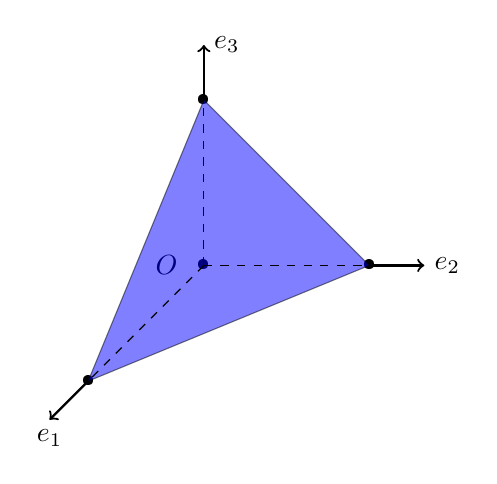
\begin{tikzpicture}[scale = .7]
        \tikzstyle{point}=[thick,draw=black,inner sep=0pt,minimum width=4pt,minimum height=4pt]

        \node (o)[label={[label distance=0cm]180:$O$}] at (0,0) {\textbullet};
        \node (a)[label={[label distance=0cm]0:}] at (3,0) {\textbullet};
        \node (b)[label={[label distance=0cm]0:}] at (0,3) {\textbullet};
        \node (c)[label={[label distance=0cm]270:}] at (-2.1, -2.1) {\textbullet};
        
        \draw[fill=blue, opacity=0.5] (a.center) -- (b.center) -- (c.center) -- cycle;
        \draw[dashed] (o.center) -- (a.center);
        \draw[dashed] (o.center) -- (b.center);
        \draw[dashed] (o.center) -- (c.center);

        \draw[thick, ->] (3,0) -- (4,0) node[anchor=west]{$e_2$};
        \draw[thick, ->] (0,3) -- (0,4) node[anchor=west]{$e_3$};
        \draw[thick, ->] (-2.1, -2.1) -- (-2.8, -2.8) node[anchor=north]{$e_1$};
    \end{tikzpicture}
    \caption{\emph{A 3D simplex where the surface of interest is enlightened.}}
    \label{fig:threeSimplex}
\end{figure}
It is clear that, while the surface gives us the number of microstates corresponding to a fixed amount of money, the volume between a fixed value $y$ such that $0 \leq y \leq N$ and $N$ gives us the cumulative distribution of the microstates, Fig. (\ref{fig:simplexVolume}).
Defining our simplex as
\begin{equation*}
    \Delta^n(N)=\left\{x \in \mathbb{R}^n \text{ s.t. } \sum_{i = 1}^n x_i = N, x_i \geq 0\right\}
\end{equation*}
we can use the result of an article \cite{simplexSampling} in which the volume of a simplex is found as
\begin{equation}
    V_n\left(y, N\right) = \frac{\sqrt{n+1}}{n!}\left[N^n - \left(N - y\right)^n\right]
\end{equation}
\begin{figure}[ht!]
    \centering
    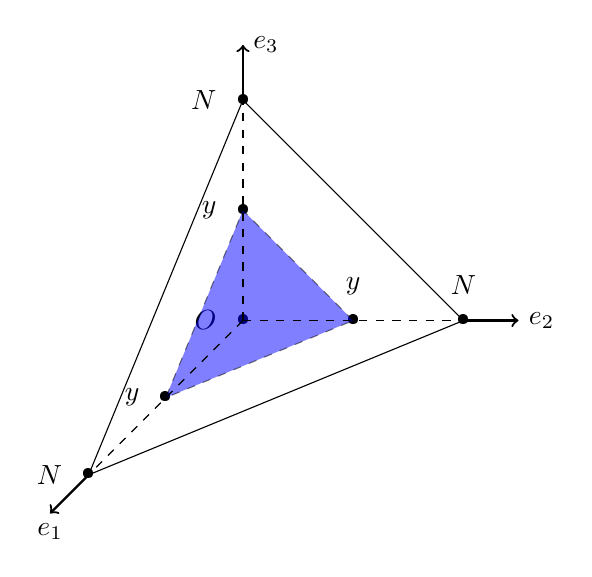
\begin{tikzpicture}[scale = .7]
        \tikzstyle{point}=[thick,draw=black,inner sep=0pt,minimum width=4pt,minimum height=4pt]

        \node (o)[label={[label distance=0cm]180:$O$}] at (0,0) {\textbullet};
        \node (a)[label={[label distance=0cm]90:$y$}] at (2,0) {\textbullet};
        \node (b)[label={[label distance=0cm]180:$y$}] at (0,2) {\textbullet};
        \node (c)[label={[label distance=0cm]180:$y$}] at (-1.4, -1.4) {\textbullet};

        \node (d)[label={[label distance=0cm]90:$N$}] at (4,0) {\textbullet};
        \node (e)[label={[label distance=0cm]180:$N$}] at (0,4) {\textbullet};    
        \node (f)[label={[label distance=0cm]180:$N$}] at (-2.8,-2.8) {\textbullet};  
        
        \draw[dashed, fill=blue, opacity=0.5] (a.center) -- (b.center) -- (c.center) -- cycle;
        \draw[dashed] (o.center) -- (d.center);
        \draw[dashed] (o.center) -- (e.center);
        \draw[dashed] (o.center) -- (f.center);
        \draw (d.center) -- (e.center) -- (f.center) -- cycle;

        \draw[thick, ->] (4,0) -- (5,0) node[anchor=west]{$e_2$};
        \draw[thick, ->] (0,4) -- (0,5) node[anchor=west]{$e_3$};
        \draw[thick, ->] (-2.8, -2.8) -- (-3.5, -3.5) node[anchor=north]{$e_1$};
    \end{tikzpicture}
    \caption{\emph{Fraction of volume of the simplex we are interested.}}
    \label{fig:simplexVolume}
\end{figure}
We want to normalize it all as we are looking for a pdf, so we can divide $V_n\left(y, N\right)$ by $V_n\left(N, N\right)$ finding the cumulative distribution
\begin{equation}
    F(y) = \frac{V_n\left(y, N\right)}{V_n\left(N, N\right)} = 1 - \left(1 - \frac{y}{N}\right)^n
\end{equation}
We note that in our case $N=\alpha n$ so
\begin{equation*}
    F(y) =  1 - \left[\left(1 - \frac{y}{\alpha n}\right)^{\alpha n}\right]^\frac{1}{\alpha}
\end{equation*}
but $n$ is the dimension of the simplex, i.e. the number of agents of the system itself.
For a great amount of agents we can take the previous relation in the limit $n\to\infty$ obtaining
\begin{equation}
    F(y) = 1 - e^{-\frac{y}{\alpha}}
\end{equation}
Now that we have the cumulative distribution of the microstate it's trivial to find the pdf applying the definition
\begin{equation*}
    f(y) = \frac{d}{dy}F(y) = \frac{1}{\alpha} e^{-\frac{y}{\alpha}}
\end{equation*}
Since we are only interested in the trend of the pdf, the result obtained can be synthesized into
\begin{equation}
    f(y) \propto e^{-\frac{y}{\alpha}}
\end{equation}
